% ----------------------------------------------------------
% Metodologia
% ----------------------------------------------------------
\chapter{Trabalhos Relacionados}

\section{“Vem Para Estância”}

O aplicativo “Vem Para Estância”, criado no município de Estância (SE), é fruto de um trabalho conjunto entre pesquisadores, gestores culturais e a própria comunidade. A ideia foi reunir e divulgar os principais patrimônios históricos e turísticos da cidade. Com o uso de geolocalização, imagens e descrições detalhadas, o app permite que o usuário conheça virtualmente pontos como monumentos, praças, igrejas e festas tradicionais, valorizando os aspectos culturais mais marcantes da região. \cite{oliveira-cultura-tecnologias-ufse}

\begin{figure}[H]
	\caption{\label{fig:cap_tela_ref_01}Captura de Tela da Página Inicial do “VEM PARA ESTÂNCIA”}
    \centering
    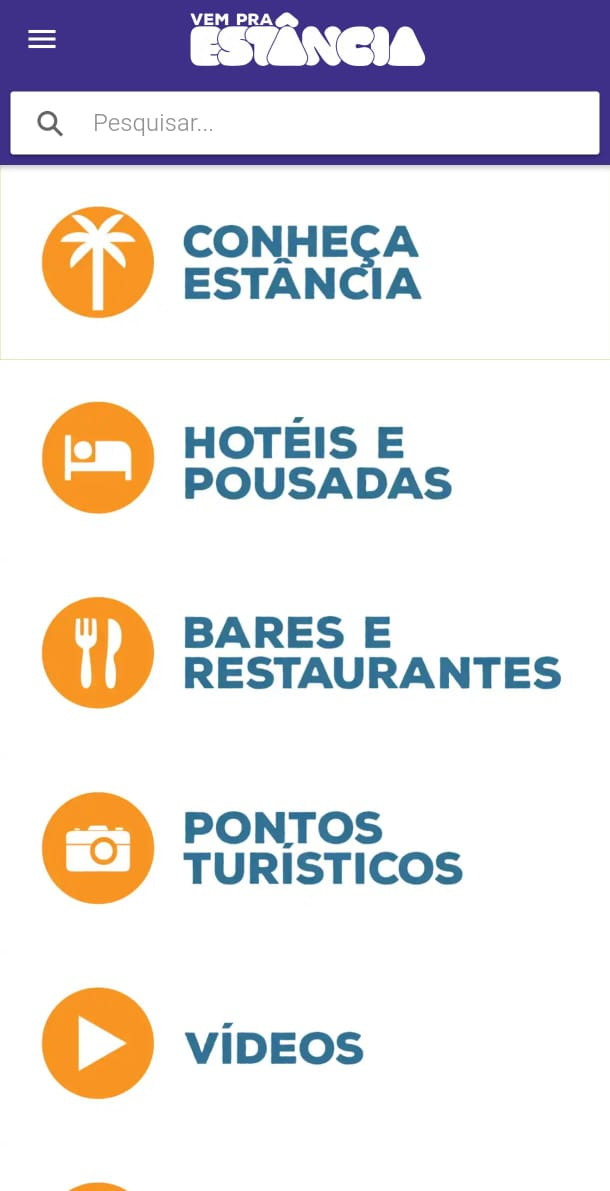
\includegraphics[scale=0.25]{imagens/Vem_Pra_Estancia3.jpeg}
    \legend{Fonte: Elaborado pelo autor a partir do aplicativo “VEM PARA ESTÂNCIA”}
\end{figure}

\begin{figure}[H]
	\caption{\label{fig:cap_tela_ref_02}Captura de Tela da Página Inicial do “VEM PARA ESTÂNCIA”}
    \centering
    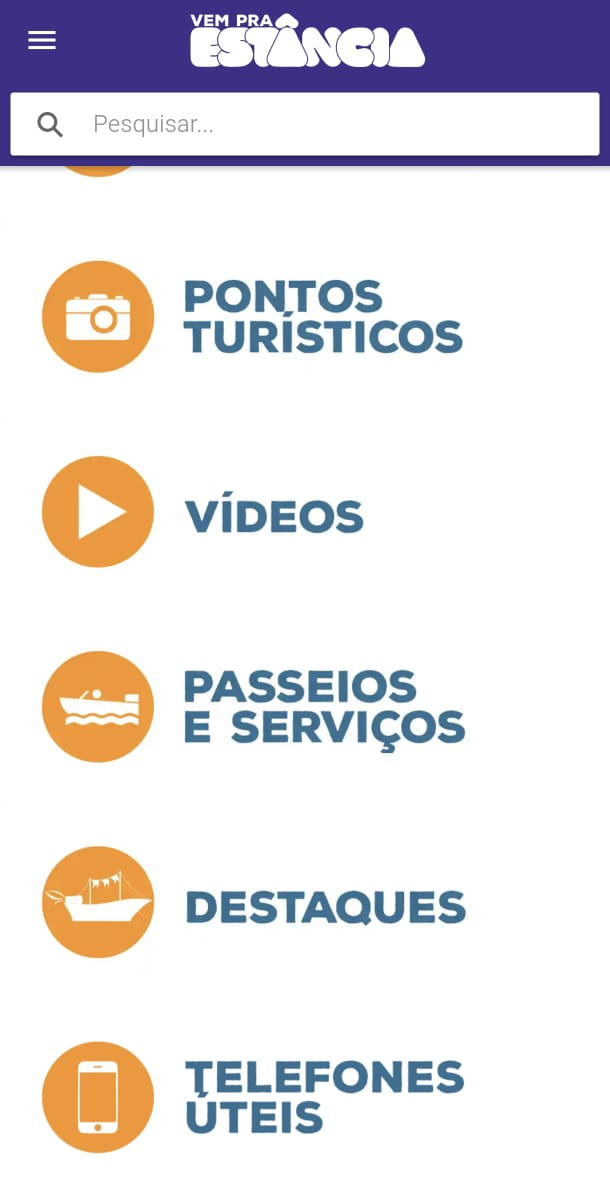
\includegraphics[scale=0.25]{imagens/Vem_Pra_Estancia2.jpeg}
    \legend{Fonte: Elaborado pelo autor a partir do aplicativo “VEM PARA ESTÂNCIA”}
\end{figure}

\begin{figure}[H]
	\caption{\label{fig:cap_tela_ref_03}Captura de Tela de Pontos Turisticos}
    \centering
    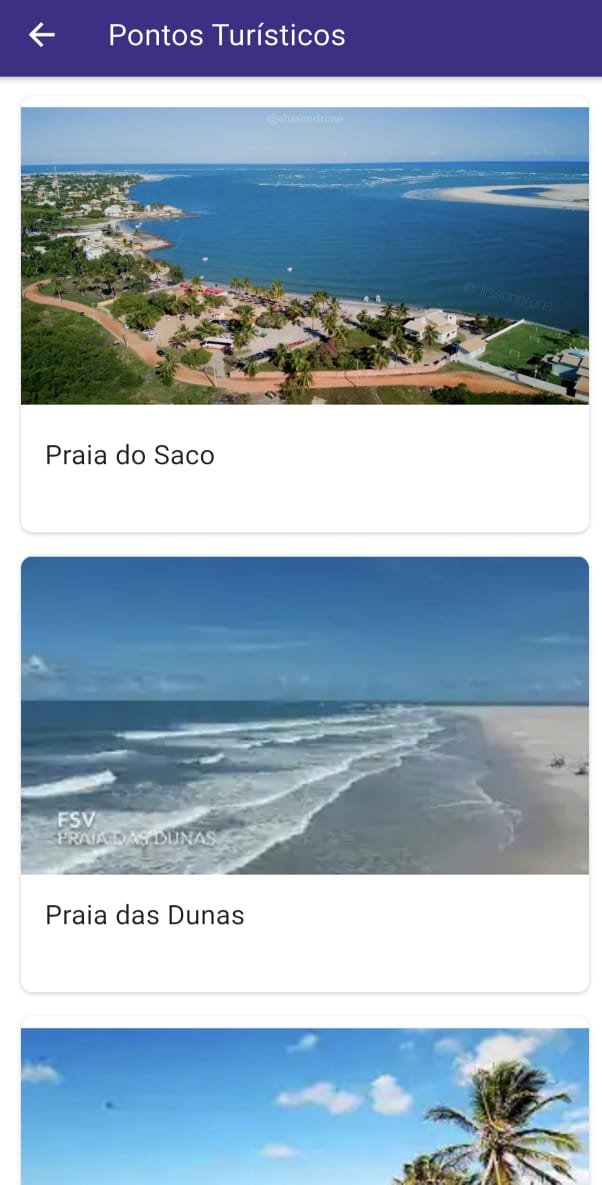
\includegraphics[scale=0.25]{imagens/Vem_Pra_Estancia1.jpeg}
    \legend{Fonte: Elaborado pelo autor a partir do aplicativo “VEM PARA ESTÂNCIA”}
\end{figure}

Mais do que apenas informar, o aplicativo também oferece uma experiência interativa. Ele permite que moradores e visitantes participem ativamente, sugerindo novos pontos culturais ou atualizando informações já cadastradas. Essa participação ajuda a criar um sentimento de pertencimento e colaboração, fortalecendo o vínculo entre a comunidade e seu patrimônio. Como resultado, foi observado um maior interesse pela história local e um engajamento crescente de diferentes públicos nas ações culturais promovidas pela cidade.

Esse exemplo tem relação direta com o projeto em desenvolvimento aqui, pois ambos propõem o uso de um aplicativo móvel com foco na participação da comunidade, uso de geolocalização, e registro visual e textual de pontos culturais. Assim como o “Vem Para Estância”, a proposta atual também busca democratizar o acesso à cultura, valorizar identidades locais e permitir que os próprios usuários atuem como agentes ativos na preservação e divulgação do patrimônio de seus territórios.

\section{Aplicativos com Realidade Aumentada e Gamificação}

O uso de realidade aumentada (RA) e gamificação tem se tornado uma estratégia cada vez mais comum em aplicativos culturais, especialmente para atrair o público jovem e promover o interesse pelo patrimônio histórico. Em várias cidades, já existem aplicativos que usam a câmera do celular para mostrar informações digitais sobre monumentos, ruas antigas ou locais históricos. Com isso, o usuário pode ver reconstruções em 3D, vídeos ou outros conteúdos interativos que tornam a visita mais rica e interessante. \cite{soster2021tecnologias}

Esse tipo de recurso ajuda não só a atrair novos públicos, mas também a tornar o aprendizado sobre cultura e história mais divertido e acessível. A gamificação com desafios, conquistas e rankings estimula as pessoas a explorarem a cidade e seus pontos culturais, despertando o senso de pertencimento e incentivando o aprendizado fora da sala de aula. Além disso, iniciativas assim também têm impacto positivo no turismo local e na economia criativa, ajudando a divulgar manifestações culturais que antes eram pouco conhecidas.

O projeto apresentado aqui ainda não utiliza realidade aumentada, mas se aproxima dessas propostas ao buscar tornar o acesso à cultura mais envolvente e acessível. Com recursos como geolocalização, imagens, textos informativos e opções de acessibilidade, o aplicativo já oferece uma base sólida que pode ser expandida futuramente para incluir novas tecnologias que aumentem ainda mais o engajamento e a valorização da cultura regional.

\section{Plataformas Públicas de Mapeamento Cultural}

Plataformas públicas como o Mapa da Cultura \cite{mapa_cultura} e os sistemas ligados ao programa Cultura Viva \cite{cultura_viva_programa} têm tido um papel importante na organização e divulgação do patrimônio cultural brasileiro. Normalmente desenvolvidos por órgãos públicos em parceria com universidades ou coletivos culturais, esses sistemas permitem que qualquer pessoa possa cadastrar espaços, eventos e grupos culturais, criando um banco de dados colaborativo e aberto ao público. \cite{prolam-cultura-viva-2025} \cite{nic-cultura-tecnologias-no-brasil}

O maior impacto dessas plataformas está na democratização da informação cultural. Como qualquer cidadão pode registrar dados, incluir eventos ou sugerir novos pontos, há uma chance real de dar visibilidade a expressões culturais periféricas ou tradicionais que, muitas vezes, ficam de fora das políticas públicas mais centralizadas. Isso fortalece o papel das comunidades na construção da memória coletiva e cria oportunidades para novas redes de apoio, divulgação e até financiamento cultural.

O aplicativo que está sendo desenvolvido neste trabalho segue uma lógica parecida. Ele também propõe a participação ativa dos usuários no cadastro dos pontos culturais, com a adição de filtros regionais, registros visuais e informações sobre acessibilidade. A intenção é tornar o conteúdo mais representativo da diversidade local e, com isso, contribuir para a valorização das identidades regionais e o acesso mais justo e democrático à cultura.

\section{Considerações sobre os Trabalhos Relacionados}

A análise dos exemplos apresentados mostra que o uso de aplicativos e plataformas digitais já se consolidou como uma estratégia bastante útil para democratizar o acesso à cultura e reforçar as identidades locais. No entanto, também fica claro que o sucesso dessas iniciativas depende de alguns pontos importantes, como a facilidade de navegação nos aplicativos, a presença de recursos acessíveis como mapas, imagens, filtros regionais e principalmente, o envolvimento da comunidade no processo de inserção e validação das informações.

Esses aspectos foram levados em consideração na construção do aplicativo desenvolvido neste projeto. A proposta buscou seguir essas boas práticas observadas nos trabalhos analisados, integrando elementos que facilitam o uso, ampliam a acessibilidade e estimulam a participação ativa dos usuários. Dessa forma, o aplicativo se alinha às estratégias mais eficazes já aplicadas em outras iniciativas culturais, fortalecendo seu potencial de impacto local.